\documentclass{beamer}
\usepackage{amsmath,amsfonts}	% use math symbols
\usepackage{graphicx} % insert images
\usepackage{url} % insert urls
\usepackage{textpos} % package for the positioning
\usepackage{caption}
\usepackage{subcaption}
\usepackage{mathtools}
\usetheme{Ilmenau} % change theme
%% NEW COMMANDS
\def\ci{\perp\!\!\!\perp}
\def\dep{\perp\!\!\!\perp\!\!\!\!\!\!\!/\,\,\,\,}
\begin{document}

%% MAKE TITLE
\title{Learning Causation from Data}
\subtitle{Fundamental of Casual Inference and its Applications}
\author{Huang Xiao} %\\ \small{xiaohu@in.tum.de} }%\thanks{Funded by ARAMiS project}}
%\and Author2 \inst{1} }
%\and Author3 \inst{2}}
\institute[Technische Universit\"at M\"unchen]
{ 
	%\inst{1} 
	Chair of IT Security (I20) \\Department of Informatics \\Technische Universit\"at M\"unchen 
	%\and
	%\inst{2} Cloud Service Lab\\Fraunhofer AISEC
}

\date{\today}
\maketitle

%% CHANGE THE DEFAULT TEMPLATE
% position the logo
\addtobeamertemplate{frametitle}{}{%
\begin{textblock*}{100mm}(0.98\textwidth,-0.7cm)

\includegraphics[height=0.53cm,width=0.9cm,keepaspectratio]{imgs/TUM}
\end{textblock*}}

\AtBeginSection[] {
	\frame<beamer>{ 
		\frametitle{Overview}   
		\tableofcontents[currentsection] 
 	}
 }
 % add frame number
%\setbeamertemplate{footline}{%
  %\raisebox{5pt}{\makebox[\paperwidth]{\hfill\makebox[10pt]{\scriptsize\insertframenumber}}}}

%% START PRESENTATION
\section{Fundamental of Causal Inference}
\subsection{Motivation}
\begin{frame}{What is Causality?}
\begin{block}{A definition from Wikipedia}
\textbf{Causality} (also referred to as causation) is the relationship
between an event (\textit{the cause}) and a second event (\textit{the effect}),
where the second event is understood as a consequence of the
first.
\end{block}\pause
\textbf{An example in real life} : Does smoking cause lung cancer?\\
\pause	
\begin{center}
\alert{Yes, it might be!}
\end{center}
\end{frame}
\begin{frame}{From Probabilistic View }
\textbf{Problem:} Does smoking cause lung cancer?\pause
\begin{center}
\begin{itemize}
\item Smoking does \alert{increase the probability} of getting lung cancer.
\end{itemize}
\end{center}
\end{frame}
\begin{frame}{Statistical Inference Overview}
\begin{figure}
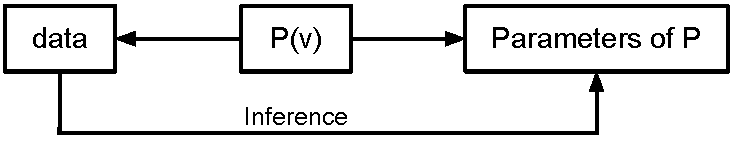
\includegraphics[scale=0.7]{imgs/statInf}
\end{figure}
\begin{itemize}
\item Approximate an estimate of $X$ given evidence $e$, namely, $Pr(X\,|\,e)$. E.g., Regression or Classification problems.
\item Rejection of hypothesis, i.e., assert wether samples are from a certain distribution.  
\item Confidence interval, i.e., construct an interval based on dataset 
\end{itemize}
\end{frame}
\begin{frame}{Causal Inference Overview}
\begin{figure}
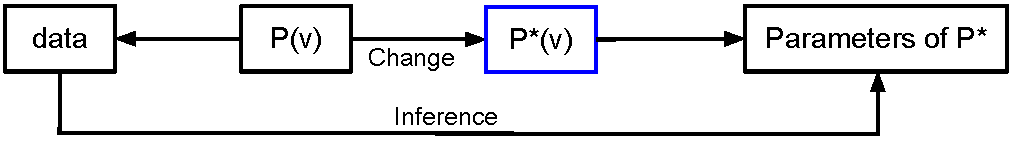
\includegraphics[scale=0.6]{imgs/causalInf}
\end{figure}
\begin{itemize}
\item What if $P$ has shifted itself to $P^*$?
\item<2-> \textbf{Key factors:} Causes, Changes, and Invariants . 
\item<2-> Inference of $P^*$ and reasoning of changes. 
\end{itemize}
\end{frame}
\begin{frame}{What makes Causal Inference interesting?}
\begin{itemize}
\item Human understands the world in terms of causes and effects.
\item Empirical science is about establishing causes.
\item Causal inference gives a mathematical language for causal
statements, and tools to solve causal problems formally.
\item Alternative exercising to decision making, reasoning, etc.
\end{itemize}
%\begin{alertblock}{Note}
%Causal Inference has fundamental difference with machine learning
%\end{alertblock}
\end{frame}
\subsection{Causal Graphical Model}
\begin{frame}{Association}
\begin{itemize}
\item Now we want to find out what \alert{causes} lung cancer
\end{itemize} \pause
\begin{columns}
\begin{column}{0.5\textwidth}
\begin{table}
\centering
\begin{tabular}{|c|c|c|c|}
\hline
& & \multicolumn{2}{|c|}{Lung cancer}\\\hline
smoking & yellow teeth & yes & no\\\hline
yes & yes & 100 & 400\\\hline
yes & no & 100 & 400\\\hline
no & yes & 1 & 450\\\hline
no & no & 9 & 8540\\\hline
\end{tabular}
\caption{Data observations from 10000 people}
\end{table}
\end{column}\hfill
\begin{column}{0.5\textwidth}
\vspace*{-0.5in}
\begin{figure}
\centering
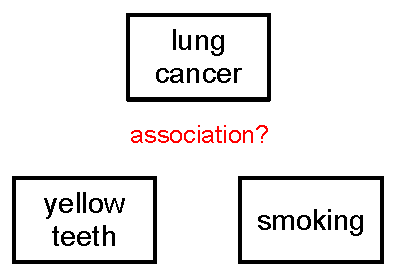
\includegraphics[scale=0.6]{imgs/smokepl}
\end{figure}
\end{column}
\end{columns}
\end{frame}
\begin{frame}{Measurements of Association}
\textbf{To find out associations among variables}
\begin{itemize}
\item Mutual information (Information theory)
\item Pearson (linear) correlation
\item Spearman's rho (rank correlation)
\item Effect size between two variables
\item Many others
\end{itemize}
\end{frame}
\begin{frame}{Observations from Data}
\textbf{Obviously}
\begin{itemize}
\item \textit{yellow teeth} and \textit{lung cancer} are associated.
\end{itemize}\pause
\alert{\textbf{But...}}
\begin{itemize}
\item Bleaching the teeth does not help reduce the probability
of getting lung cancer.
\end{itemize}\pause
\begin{alertblock}{Caution!}
Correlation does not imply Causation
\end{alertblock}
\end{frame}
\begin{frame}{Statistical Implication}
\begin{block}{Reichenbach's \textit{Common Cause Principle}}
If $X$ and $Y$ are correlated, then either $X$ causes $Y$ or $Y$ causes $X$ or they share a latent common cause $Z$.
\end{block}
\begin{figure}
\setcounter{subfigure}{0}
	\centering
	\begin{subfigure}[H]{0.3\textwidth}
		\centering
		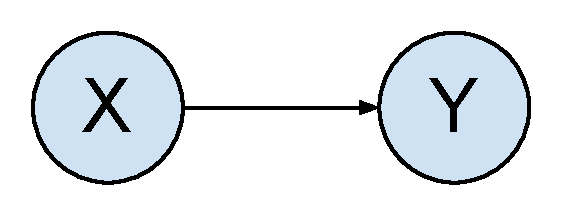
\includegraphics[scale=0.3]{imgs/x2y}
		\caption{$X$ causes $Y$}
		%\label{}	
	\end{subfigure}
	\begin{subfigure}[H]{0.3\textwidth}
		\centering
		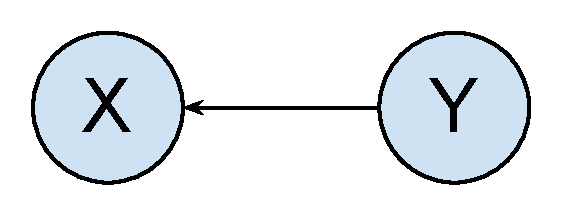
\includegraphics[scale=0.3]{imgs/y2x}
		\caption{$Y$ causes $X$}
		%\label{}	
	\end{subfigure}
	\begin{subfigure}[H]{0.3\textwidth}
		\centering
		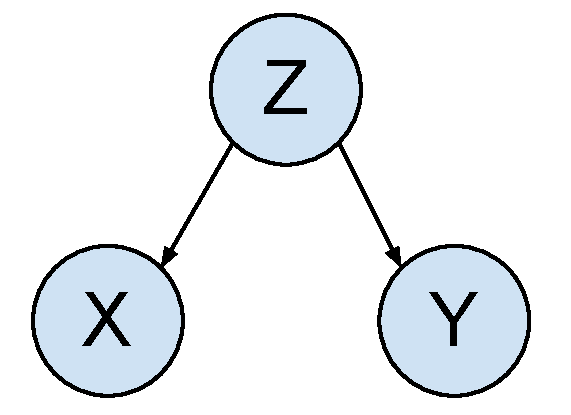
\includegraphics[scale=0.3]{imgs/z2xy}
		\caption{A common latent cause $Z$}
		%\label{}	
	\end{subfigure}
\end{figure}\pause
\begin{itemize}
\item<+-|alert@+> It links causality with probability
\end{itemize}
\end{frame}
\begin{frame}{Functional Causal Model (pearl et al.)} 
\begin{itemize}[<+->]
\item A set of variables (factors) $\left\lbrace X_1,\ldots,X_n \right\rbrace$
\item Directed acyclic graph $\mathcal{G}$ with vertices $\left\lbrace X_1,\ldots,X_n \right\rbrace$
\item Parents of node $X_i$ in $\mathcal{G}$ are its direct causes
\item $X_i=f_i(Parents(X_i),\epsilon_i)$, where $\left\lbrace\epsilon_1,\ldots,\epsilon_n\right\rbrace$ are jointly independent noises
\item The above entails a joint probability distribution $P(X_1,\ldots,X_n)$
\item Problems are twofold:
      \begin{enumerate}
		\item How is the $P$ like?
		\item Can we recover $\mathcal{G} from P$? 
	\end{enumerate}
\item[] \begin{textblock*}{200mm}(0.6\textwidth,-2cm)
		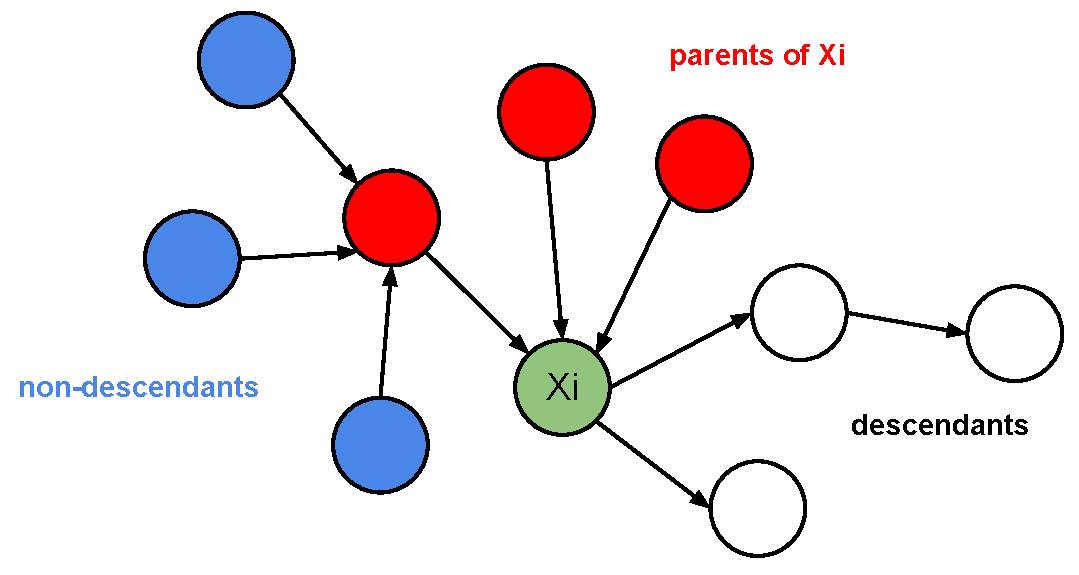
\includegraphics[scale=0.25]{imgs/causalgm}
	\end{textblock*}
\end{itemize}
\end{frame}
\begin{frame}{Functional Causal Model, ctd.}
The following are equivalent:
\begin{itemize}
\item A functional causal model exists
\item Local causal Markov condition: $X_i$ is statistically independent of its non-descendants given $X_i$'s parents
\item Global Causal Markov condition: \textbf{d-separation} characterize the set of independences over all the observables
\item Factorization: $P(X_1,\ldots,X_n)=\prod_iP(X_i\,|\,Parents(X_i))$
\end{itemize}
\end{frame}
\begin{frame}{Learning causation from Data?}
\begin{block}{Question}
Given observational data, can we infer $\mathcal{G}$?
\end{block}
\begin{itemize}
\item \textbf{Simple answer:} impossible without additional information
\item Possible with interventions (outside force, empirical treatment, etc.)
\item By conditional independence tests, \textit{Markov equivalence class} containing $\mathcal{G}$ can be learned. \alert{But}, it fails in simplest 2-nodes case.
\item 2-nodes case can be tackled applying residual dependence test. (see Hoyer et al.)
\end{itemize}
\end{frame}
\begin{frame}{Markov Equivalence Class}
\textbf{Simplest case with three variables}
\begin{itemize}
\item[]<1-> \begin{figure}
\setcounter{subfigure}{0}
			\begin{subfigure}[H]{0.4\textwidth}
			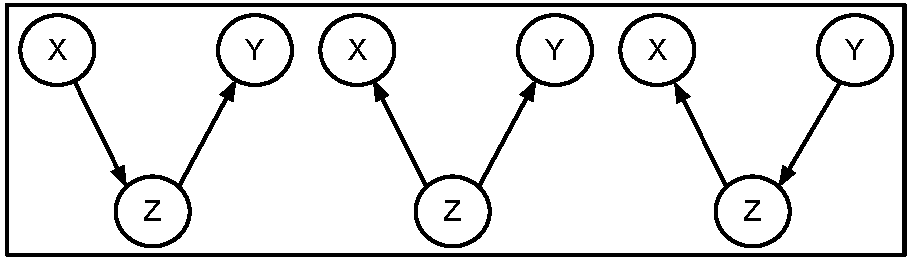
\includegraphics[scale=0.4]{imgs/eqv}
			\caption{Equivalence}
			\end{subfigure}\hfill
			\begin{subfigure}[H]{0.3\textwidth}
			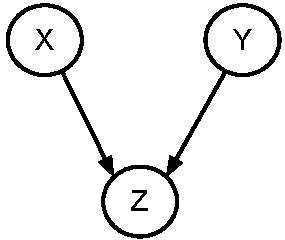
\includegraphics[scale=0.4]{imgs/noneqv}
			\caption{Non-equivalence}
			\end{subfigure}
		\end{figure}
\item<2-> Samples can be explained by all graphs in equivalence class
\item<3-> For example:
\begin{table}
\centering
\begin{tabular}{|c|c|}
\hline
Equivalence class & Non-equivalence class \\\hline
$Dep(X,Z\,|\,\emptyset)$ & $Dep(X,Z\,|\,\emptyset)$\\\hline
$Dep(Y,Z\,|\,\emptyset)$ & $Dep(Y,Z\,|\,\emptyset)$\\\hline
$Dep(X,Y\,|\,\emptyset)$ & \alert{$Ind(X,Y\,|\,\emptyset)$}\\\hline
$Ind(X,Y\,|\,Z)$ & \alert{$Dep(X,Y\,|\,Z)$}\\\hline
\end{tabular}
\end{table}	
\end{itemize}
\end{frame}
%% START NEW SECTION
\section{Causal Bayesian Network}
\subsection{Background and Definition}
\begin{frame}{Assumptions}
\begin{itemize}[<+->]
\item Causal Markov Condition
	\begin{itemize}
	\item Every variable is independent of its non-descendants given its parents
	\item Factorization: $P(X_1,\ldots,X_n)=\prod_iP(X_i\,|\,Parents(X_i))$
	\end{itemize}
\item Faithfulness: causal structure fully determines independences
\item Acyclic: needs to be defined in problem setting
\item Causal sufficiency
	\begin{itemize}
	\item Assume no latent common cause
	\item For efficient learning, also for causal interpretation of output
	\end{itemize}
\end{itemize}
\end{frame}
\begin{frame}{Causal Bayesian Network}
\begin{definition}
Given a set of variables ${X_1,\ldots, X_n}$, a Bayesian network is
a probabilistic graphical model $B = (\mathcal{G}, \Theta)$, where $\mathcal{G}=(V,E)$ is a
directed acyclic graph (DAG) and $\Theta$ is the set of the
parameters in all conditional probability distributions (CPDs).
\end{definition}
A Bayesian network $B$ is said to be causal when do intervention on any subset $X\subseteq V$, i.e., do(X), 
resulting in a set of interventional distributions $P_x$, denoted by $P_*$, and the following three conditions hold:
\begin{itemize}
\item $P_x$ is Markov relative to $\mathcal{G}$
\item $P_x(v_i)=1$ for all variables $v_i\in X$
\item $P_x(v_i\,|\,pa_i)=P(v_i|pa_i)$ for all variables $v_i\notin X$
\end{itemize} 
\end{frame}
\begin{frame}{An example}
\begin{figure}
\centering
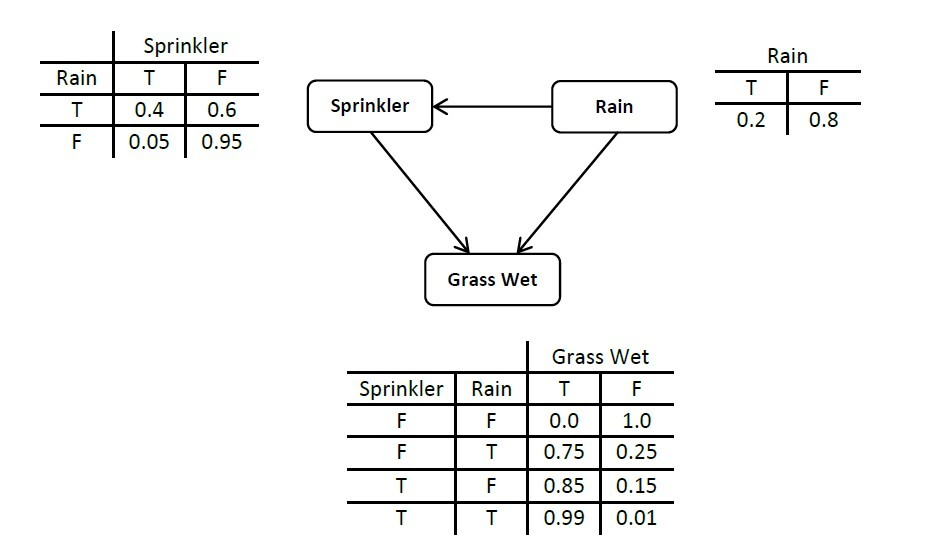
\includegraphics[scale=0.4]{imgs/bnexample}
\end{figure}
\end{frame}
\subsection{Learning Bayesian Network}
\begin{frame}{Problem Setting}
\begin{block}{Goal}
Given a dataset $\mathcal{D}$, try to learn the graph $\mathcal{G}$ and the
parameters of all conditional probability distribution $\Theta$.
\end{block}\pause
\begin{itemize}
\item[] \textbf{Traditional method}
	\item First step: structure learning
	\item Second step: parameter estimation conform to the inferred structure 
\end{itemize}
\end{frame}
\begin{frame}{Structure learning}
\begin{columns}
\begin{column}[t]{5cm}
\textbf{Constraint based}\\
Run conditional independence tests in 
data and find a DAG faithful to 
them. 
\begin{itemize}
\item \textit{Methods:} SGS, PC, TPDA, CPC 
\end{itemize}
\textbf{Hybrid}\\
Combining both constraint based and score based.
\begin{itemize}
\item \textit{Methods:} MMHC, CB, ECOS
\end{itemize}
\end{column}
\begin{column}[t]{5cm}
\textbf{Score based}\\
Find a DAG by maximizing the
posteriori probability given the data.
\begin{itemize}
\item \textit{Methods:} K2, Sparse Candidate, GBPS, BIC/AIC
\end{itemize}
\end{column}
\end{columns}
\end{frame}
\begin{frame}{Parameter Estimation}
Given the structure $\mathcal{G}$ learned from last step, factorization
will be applied according to local terms governed by parameters $\theta_i$
\begin{center}
$P(X_1,\ldots,X_n)=\prod_iP(X_i\,|\,Pa_i, \theta_i)$
\end{center}
Any parameter estimator will work here, e.g, MLE, MAP
\end{frame}
\begin{frame}{Some problems in BN Learning}
\begin{itemize}
\item Search space is exponentially large in high dimension
\item Too many conditional tests
\item Local minimum
\item Parametric form needed
\item Missing values
\item Latent variables
\item Hybrid node type
\end{itemize}
\end{frame}
\section{A Copula-based Learning Approach}
\subsection{Copula theory}
\begin{frame}{Copula functions}
\begin{definition}
Let $U_1,\ldots,U_N$ be real random variables marginally uniformly distributed over $\left[0,1\right]$. A Copula function C is a cumulative joint probability function: $\left[0,1\right]^N \rightarrow \left[0,1\right]$.
\[
C\left(u_1,\ldots ,u_N\right)=P\left(U_1\leq u_1,\ldots ,U_N\leq u_N\right)
\]
\end{definition}	
A Copula function $C$ can be viewed as a probability function of points
distribution in a $N$-dimensional unit hypercube.
\end{frame}
\begin{frame}{Sklar's theorem}
Copula function is important because of the Sklar's theorem
\begin{theorem}[Sklar 1959]
Let $F\left(x_1,\ldots,x_N\right)$ be any cumulative multivariate distribution over real-valued random variables, then there exists a copula function $C$ such that
\begin{center}
$F\left(x_1,\ldots,x_N\right) = C\left(F\left(x_1\right),\ldots,F\left(x_N\right)\right)$,
\end{center}
where $F\left(X_i\right)$ is marginal cumulative density distribution
of variable $X_i$ and furthermore if each $F\left(X_i\right)$ is continuous then the Copula is unique.
\end{theorem}
\end{frame}
\begin{frame}{Copula Multivariate Modelling}
\textbf{Advantages}
\begin{itemize}
\item Total independent free choice of marginal distributions
\item Ability of transforming any joint distribution into a specific parametric form
\item Decrease the number of paramters to be estimated dramatically 
\item Non-parametric estimators are allowed on marginals
\end{itemize}\pause
\textbf{Multivariate modelling by Copula functions}
\begin{enumerate}[<+->]
\item Finding univariate marginals via either parametric or non-parametric ways
\item Defining a Copula function to capture the dependence structure of model
\end{enumerate}
\end{frame}
\begin{frame}{Gaussian Copulas}
\textbf{Gaussian Copula} is a widely used Copula function because of its extensive practical importance in many fields and also for computational simplicity. It has the form as follows: 
\begin{center}
$C\left(\left\lbrace F\left(x_i\right)\right\rbrace\right) = \Phi_\Sigma\left(\phi^{-1}\left(F\left(x_1\right)\right),\ldots,\phi^{-1}\left(F\left(x_n\right)\right)\right)$
\end{center}
where $\phi$ is standard normal distribution, $\Phi_\Sigma$ is zero mean normal distribution with correlation matrix $\Sigma$. \\
Other Copulas like Archimedean Copulas, Clayton Copulas, Vine Copula Models are also well studied.
\end{frame}
\begin{frame}{Gaussian Copulas, ctd.}
Taking the $N$-th order derivatives of $C$, we obtain the Gaussian Copula density function $c\left(\left\lbrace F\left(x_i\right)\right\rbrace\right)= $
\begin{align*}
\frac{1}{\sqrt{det\Sigma}}exp\left(-\frac{1}{2} \begin{pmatrix}
\phi^{-1}\left(F\left(x_1\right)\right)\\
\vdots\\
\phi^{-1}\left(F\left(x_N\right)\right)
\end{pmatrix}^T \left(\Sigma^{-1}-\mathbf{I}\right)\begin{pmatrix}
\phi^{-1}\left(F\left(x_1\right)\right)\\
\vdots\\
\phi^{-1}\left(F\left(x_N\right)\right)
\end{pmatrix}\right)
\end{align*}
where $\mathbf{I}$ is the identity matrix. Using Sklar's theorem, the multivariate Gaussian density distribution can be obtained. In a learning scheme, the correlation matrix $\Sigma$ is the only parameters to be estimated when univariate marginals are known from data observations. 
\end{frame}
\subsection{Gaussian Copula Bayesian Network}
\begin{frame}{Conditional Copula Density Function}
Let $x$ denote a variable and $\mathbf{y}=\{y_1,\dots ,y_k\}$ are the parents of $x$. And $f(x\,|\,\mathbf{y})$ is the conditional density function and $f(x)$ denotes the marginal density of $x$. And there exists a Copula density function $c(F(x),F(y_1),\dots ,F(y_k))$ such that: 
\[
f(x|\mathbf{y})=R_c(F(x),F(y_1),\dots , F(y_k))
\]
where $R_c$ is the Copula ratio
\begin{align*}
R_c(F(x),F(y_1),\dots , F(y_k))& \equiv \frac{c(F(x),F(y_1),\dots , F(y_k))}{\int c(F(x),F(y_1),\dots , F(y_k))f(x)dx}\nonumber\\
& =\frac{c(F(x),F(y_1),\dots , F(y_k))}{\frac{\partial^kC(1,F(y_1),\dots ,F(y_k))}{\partial F(y_1)\dots \partial F(y_k)}}
\end{align*}
and $R_c$ is defined to be 1 when $\mathbf{y}=\emptyset$. 
\end{frame}
\begin{frame}{Factorization of Copulas}
Consider again the factorization of Bayesian network: $p\left( X\right) = \prod^m_{i=1}p(x_i\,|\,\mathbf{Pa_i})$\\
Copulas can be decomposed in a similar way: 
\begin{block}{Decomposition of Copulas}
Given a directed acyclic graph $\mathcal{G}$ encoding conditional independences over $\mathcal{X}$, the Copula density $c\left(F\left(x_1\right),\ldots, F\left(x_N\right)\right)$ can also be decomposed according to $\mathcal{G}$
\[
c\left(F\left(x_1\right),\ldots, F\left(x_N\right)\right) = \prod_i R_{c_i}(F(x_i),\left\lbrace F(\mathbf{Pa_{ik}})\right\rbrace) 
\]
\end{block}
where $c_i$ is the local Copula ratio on variable $x_i$
\end{frame}
\begin{frame}{Copula Bayesian Network Model}
\begin{definition}
A Copula Bayesian Network (CBN) is a triplet $\mathcal{C}=(\mathcal{G}, \Theta_C, \Theta_f)$ encoding the joint density $f_\mathcal{X}(x)$. $\Theta_C$ is a set for all local Copula densities $c_i(F(x_i),\left\lbrace F(\mathbf{Pa_{ik}})\right\rbrace)$ and $\Theta_f$ is the set of parameters representing the univariate marginals $f(x_i)$. Then $f_\mathcal{X}(x)$ can be parameterized as
\[
f_\mathcal{X}(x)=\prod_i R_{c_i}(F(x_i),\left\lbrace F(\mathbf{Pa_{ik}})\right\rbrace)f(x_i)
\]
\end{definition}
By sharing the global univariate marginals, the hypothesis space on parameters has been largely reduced.
\end{frame}
\subsection{Learning Copula Bayesian Network}
\begin{frame}{Parameter Estimation}
In the case of Gaussian Copula, and we take the MLE method given data observations $T$. The log-likelihood can be written as:
\begin{equation*}
\ell(\theta) = \sum^{|T|}_{t=1}\ln c(F_1(x_1^t;\theta_1), \cdots ,F_N(x_N^t;\theta_N),\alpha)+\sum^{|T|}_{t=1}\sum^N_{n=1}\ln f_n(x^t_n;\theta_n)
\end{equation*}
where $\theta_i$ is the parameters of marginal distribution $x_i$ and $\alpha$ is the set of parameters governing the dependencies.
\end{frame}
\begin{frame}{Structure Learning}
For structure learning, we use the partial inverse correlation matrix (PICM) method (constraint based).\\
\textbf{Basic idea:} simply inverse the estimated covariance matrix $\Sigma$ in Gaussian Copula, and scale the diagonals as $1$.
\begin{small}
\onslide<2->{$\Sigma^{-1} =
\begin{pmatrix}
s_{1,1} & s_{1,2} & \cdots & s_{1,n} \\
s_{2,1} & s_{2,2} & \cdots & s_{2,n} \\
\vdots   & \vdots   & \ddots & \vdots \\
s_{n,1} & s_{n,2} & \cdot & s_{n,n} \\
\end{pmatrix}$}
\onslide<3->{$\xRightarrow{scale}
\begin{pmatrix}
1 & \frac{s_{1,2}}{s_{1,1}*s_{2,2}} & \cdot & \frac{s_{1,n}}{s_{1,1}*s_{n,n}} \\[0.3em]
\frac{s_{2,1}}{s_{2,2}*s_{1,1}} & 1 & \cdot & \frac{s_{2,n}}{s_{2,2}*s_{n,n}} \\[0.3em]
\vdots   & \vdots   & \ddots & \vdots \\
\frac{s_{n,1}}{s_{n,n}*s_{1,1}} & \frac{s_{n,2}}{s_{n,n}*s_{2,2}} & \cdot & 1 \\
\end{pmatrix}$}
\end{small}\\[0.5em]
\onslide<4->{\alert{If $\frac{s_{i,j}}{\sqrt{s_{i,i}*s_{j,j}}} \leq \sigma (\text{very small}) \Rightarrow X_i \ci X_j \,|\, \left\lbrace X_{q\neq i,j} \right\rbrace$}}
\end{frame}
\begin{frame}{PICM to Moral Graph}
A zero-entry in PICM implies no direct edge between two variables, we construct a moral graph accordingly, e.g., 
\begin{figure}
\setcounter{subfigure}{0}
\begin{subfigure}[H]{0.4\textwidth}
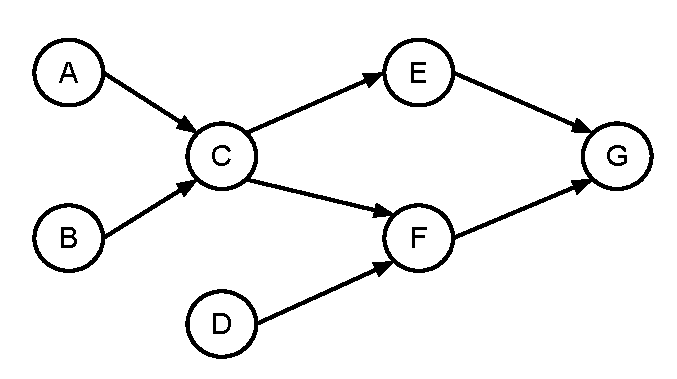
\includegraphics[scale=0.4]{imgs/BNs7n}
\caption{Original DAG}
\end{subfigure}\hfill $\Rightarrow$ \hfill
\begin{subfigure}[H]{0.4\textwidth}
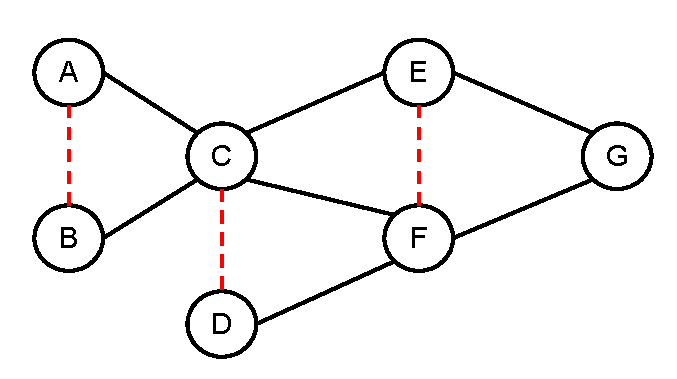
\includegraphics[scale=0.4]{imgs/BNs7nMoral}
\caption{Moral graph}
\end{subfigure}
\end{figure}
\textbf{Moral} is a term known as the married edge of the parents for a collider (two nodes converge at a common node, i.e., non-equivalence ).
\end{frame}
\begin{frame}{Detriangulation of Moral Graph}
\textbf{Note} that the additional dependences are brought by colliders (see nodes C, F, and G) and by conditioned on colliders, dependences will disappear, namely, $A\dep B \, | \, C$ but $A\ci B \,|\, \emptyset$. This motivates us to remove those additional dependences (married edges).\pause
\begin{figure}
\setcounter{subfigure}{0}
\begin{subfigure}[H]{0.4\textwidth}
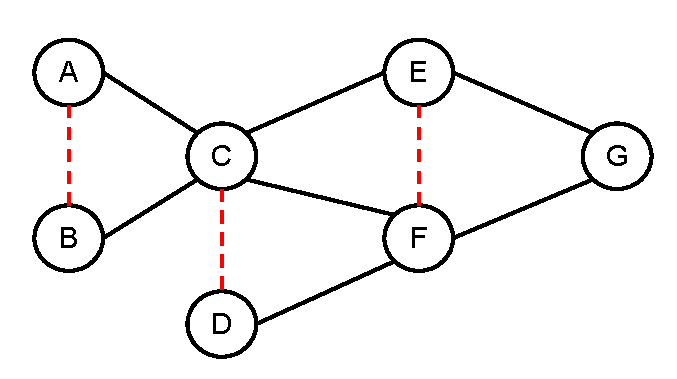
\includegraphics[scale=0.4]{imgs/BNs7nMoral}
\caption{Moral graph}
\end{subfigure}\hfill $\Rightarrow$ \hfill
\begin{subfigure}[H]{0.4\textwidth}
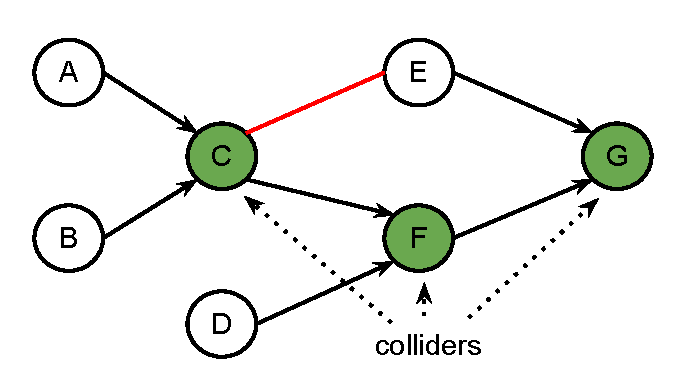
\includegraphics[scale=0.4]{imgs/BNs7nDet}
\caption{Partially directed graph after removing moral edges}
\end{subfigure}
\end{figure}
\end{frame}
\begin{frame}{Contraint Propagation (Judea Pearl 2000)}
Constraints: Colliders, Acyclicity
 \begin{figure}[H]
  \centering
  \hfill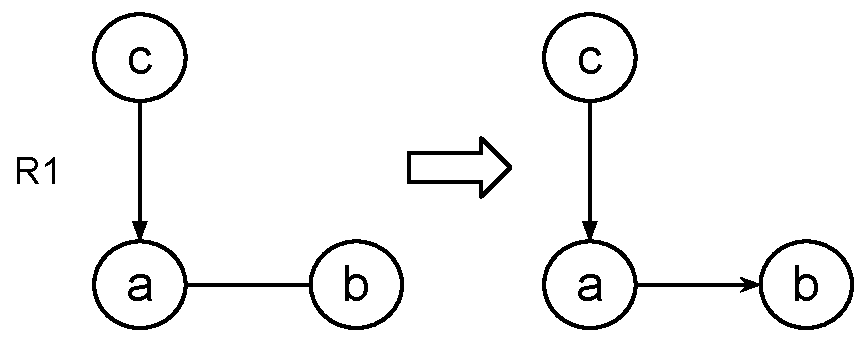
\includegraphics[width=0.4\textwidth]{imgs/R1}%      
  \hfill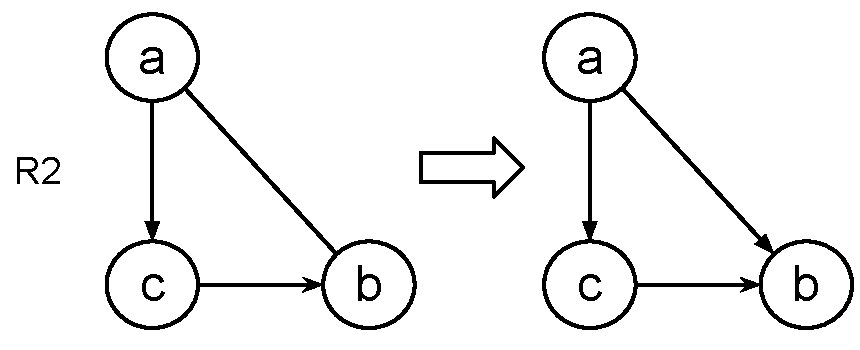
\includegraphics[width=0.4\textwidth]{imgs/R2}\hspace*{\fill}\newline
  \vspace{0.5mm}
  \hspace*{\fill}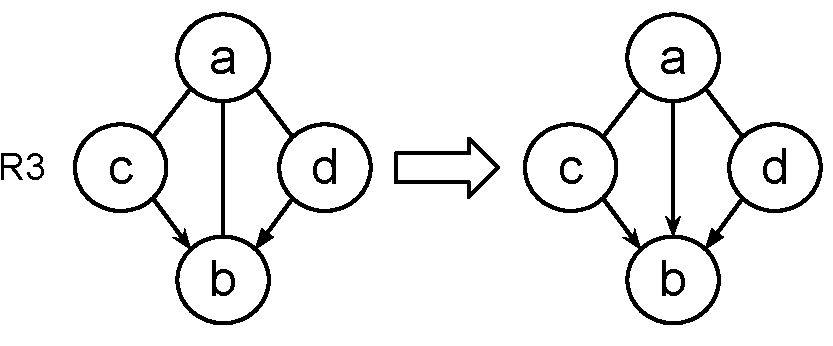
\includegraphics[width=0.4\textwidth]{imgs/R3}%
  \hfill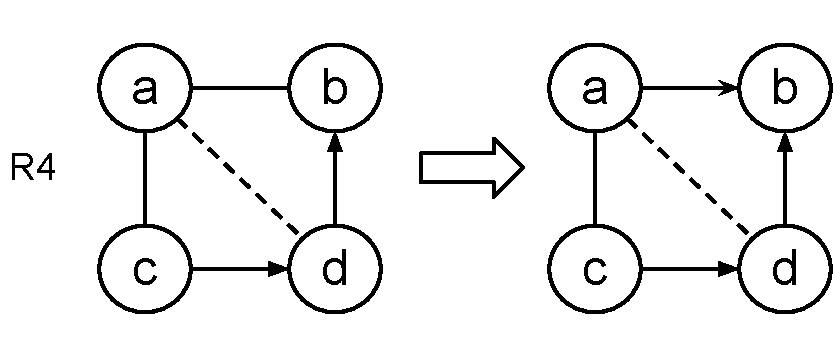
\includegraphics[width=0.4\textwidth]{imgs/R4}\hspace*{\fill}
  \caption{Rules for completion of orientations}
 \end{figure}
\end{frame}
\begin{frame}{Maximally Oriented Acyclic Graph}
Recursively propagate constraints, we obtain a maximally oriented acyclic graph (\alert{only equivalence class})
\begin{figure}
\setcounter{subfigure}{0}
\begin{subfigure}[H]{0.4\textwidth}
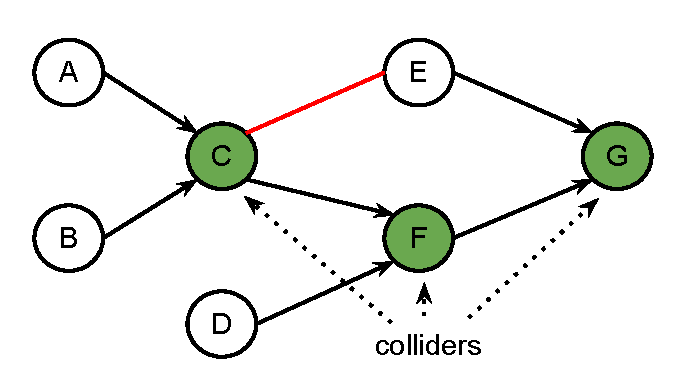
\includegraphics[scale=0.4]{imgs/BNs7nDet}
\caption{Partially directed graph after removing moral edges}
\end{subfigure}\hfill $\Rightarrow$ \hfill
\begin{subfigure}[H]{0.4\textwidth}
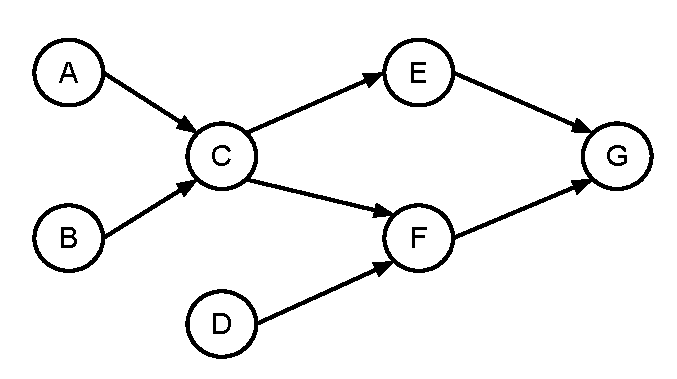
\includegraphics[scale=0.4]{imgs/BNs7n}
\caption{Maximally oriented acyclic graph}
\end{subfigure}
\end{figure}
\end{frame}
\section{Experiments}
\subsection{Synthetic Data Set}
\begin{frame}{Structural Hamming Distances}
$5$ synthetic networks of size $5,7,10,20,50$. (ground truth structures are known.)
\begin{figure}
\vspace{-2cm}
\centering
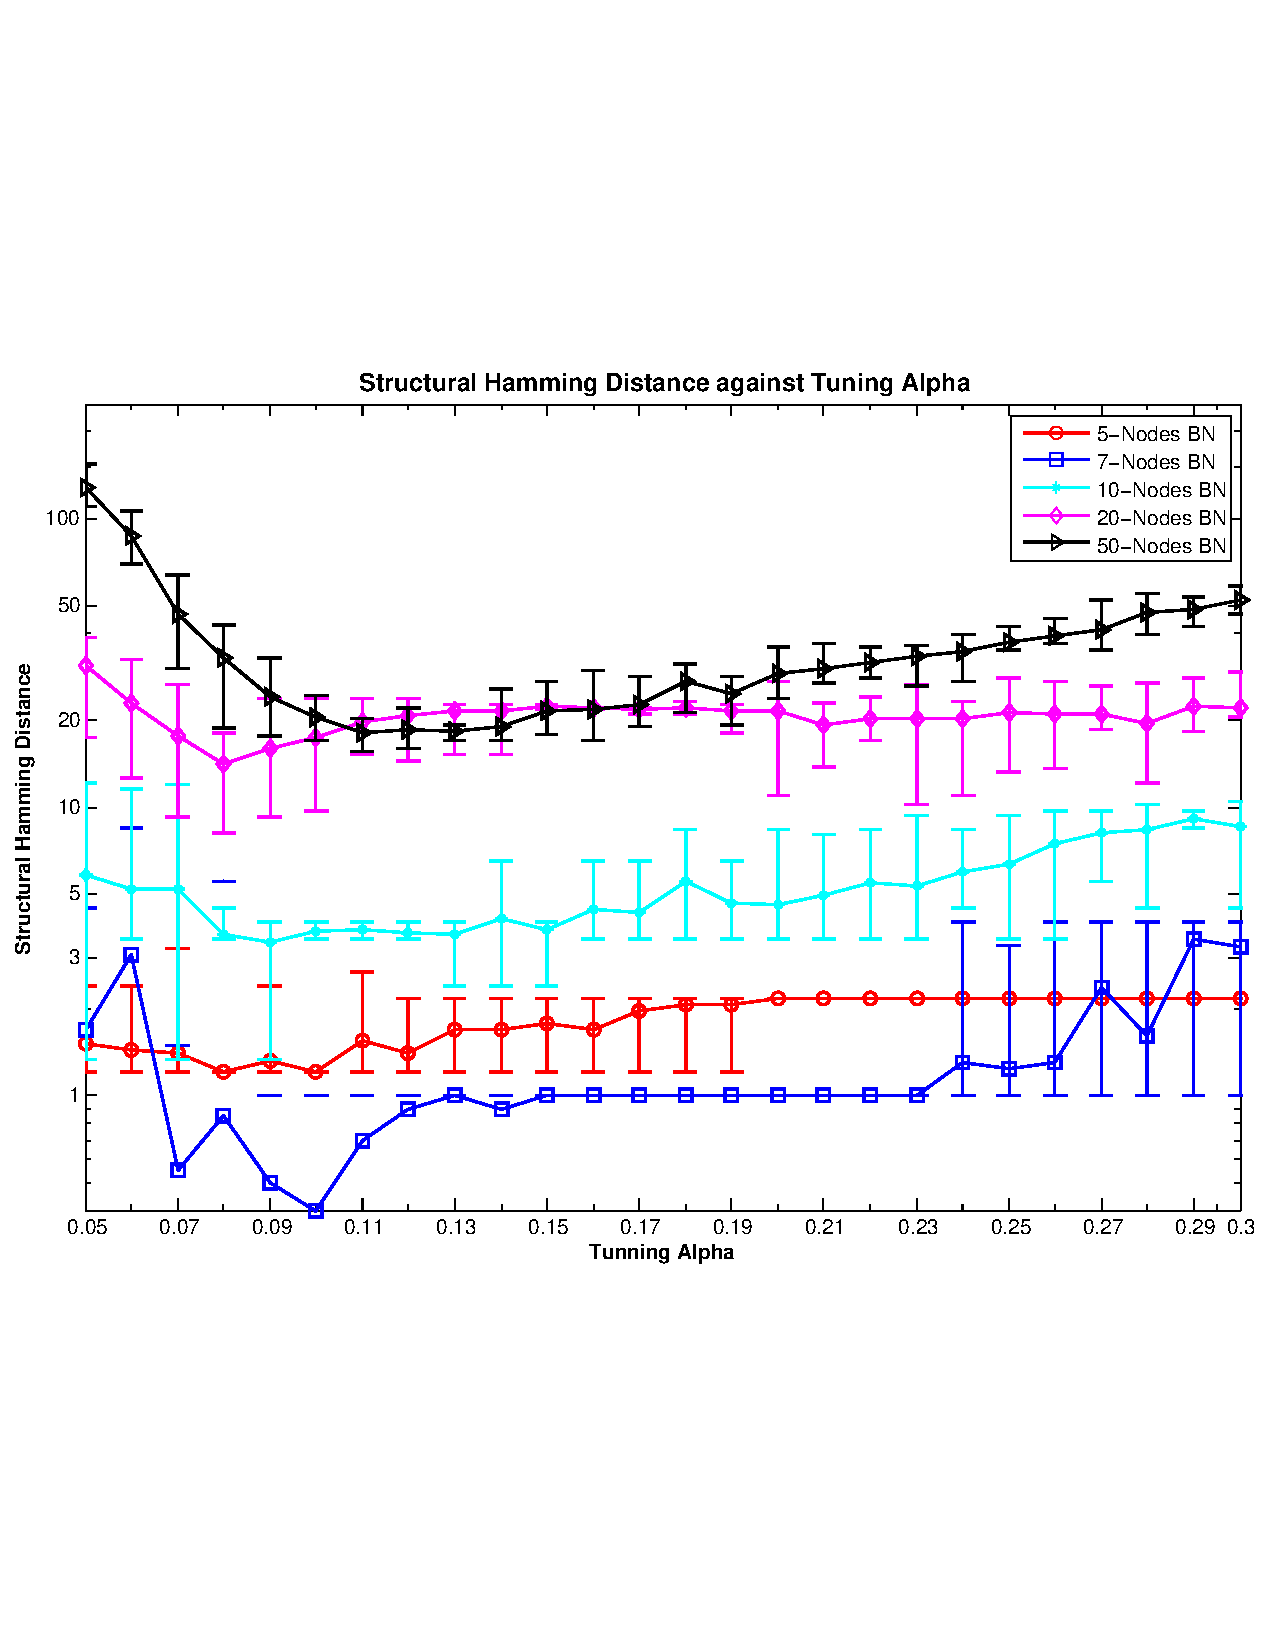
\includegraphics[scale=0.3]{imgs/shd-alpha-errb}
\vspace{-2cm}
\caption{Structural hamming distance (SHD) against threshold $\sigma$}
\end{figure} 
\end{frame}
\begin{frame}{Error rates}
\begin{figure}
\vspace{-2cm}
\centering
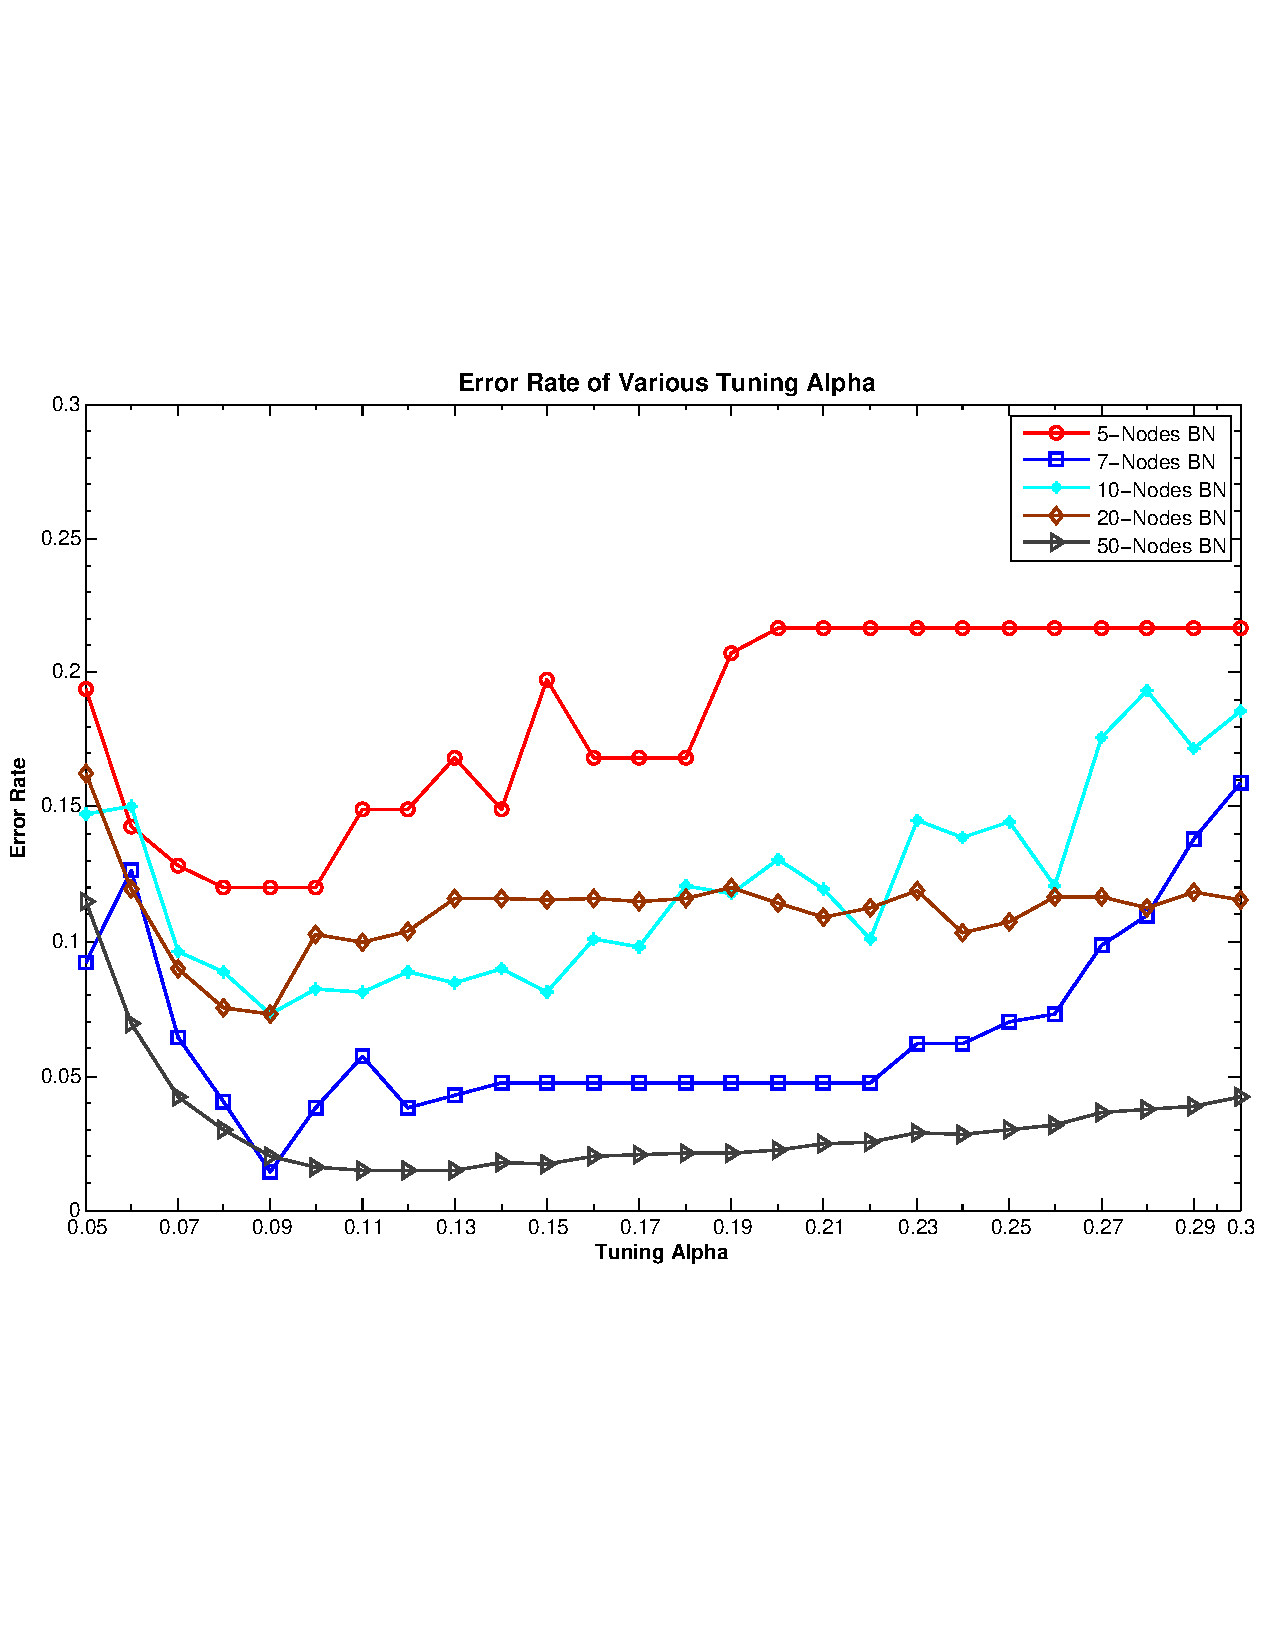
\includegraphics[scale=0.35]{imgs/ErrorRate-copula}
\vspace{-2.2cm}
\caption{Error rates in terms of SHD}
\end{figure} 
\end{frame}
\subsection{Real-world Data Set}
\begin{frame}{Boston Housing Price (UCI Repo.)}
\begin{minipage}[t]{0.45\linewidth}
 \vspace{0pt}
\centering
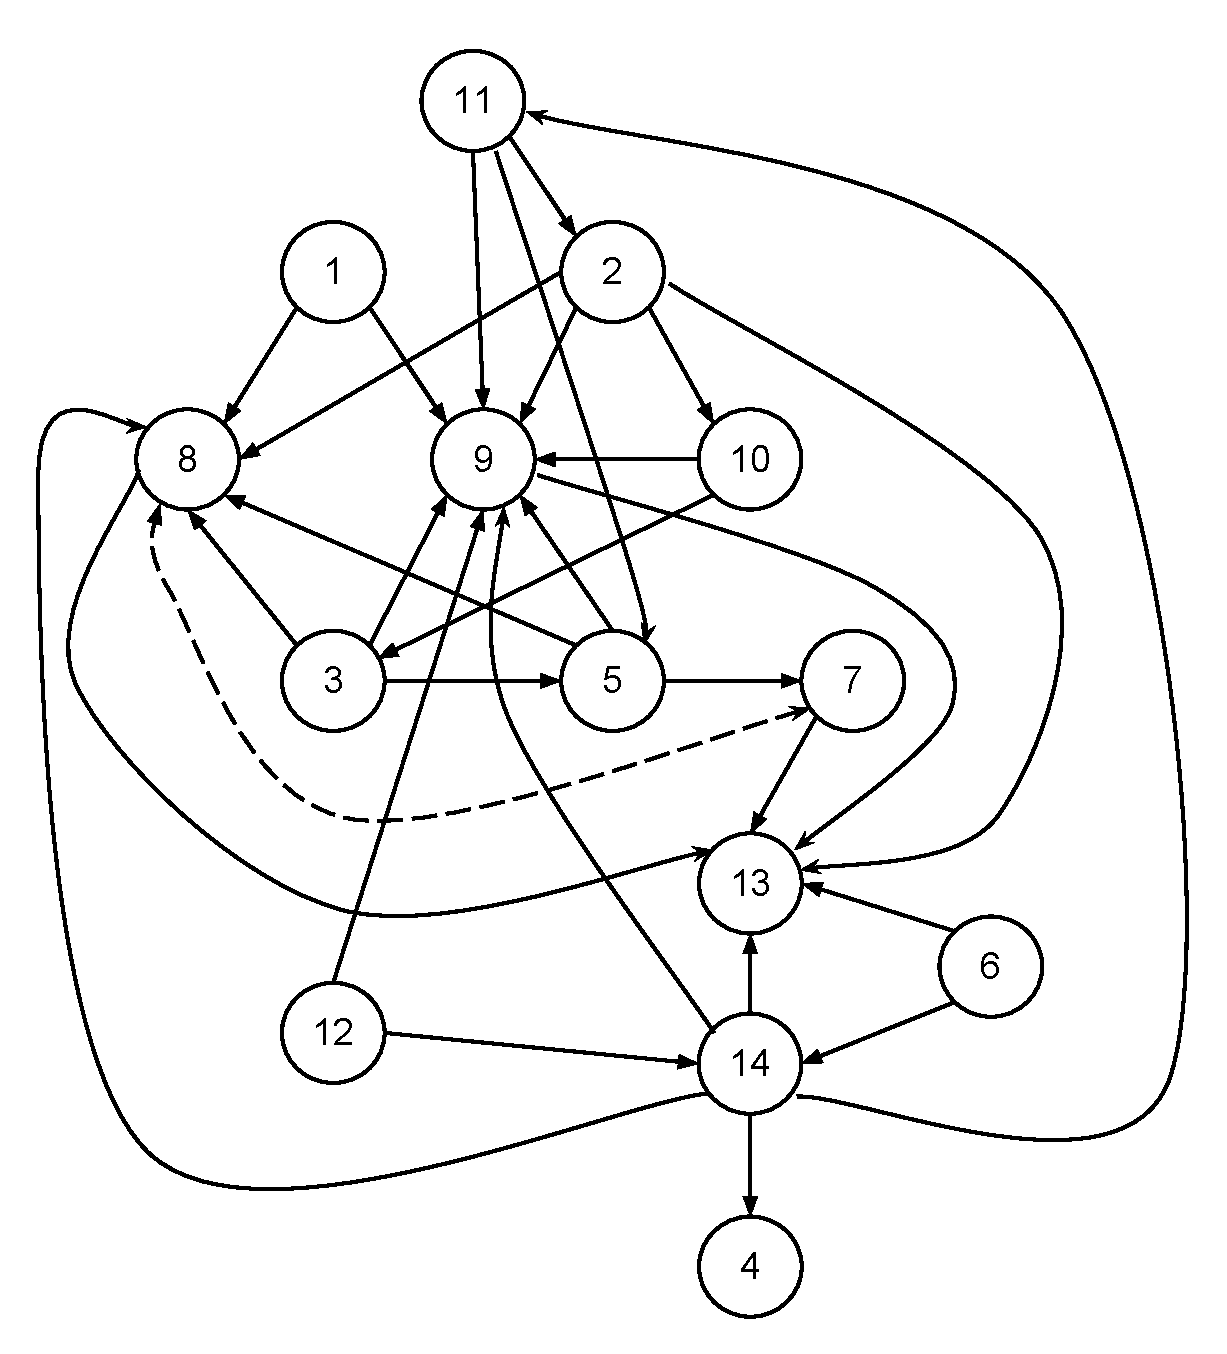
\includegraphics[width=\textwidth]{imgs/BostonHousingNetwork}
\end{minipage}\hfill
\begin{minipage}[t]{0.4\linewidth}
 \vspace{0pt}
\centering
\begin{scriptsize}
\begin{tabular}{|l|}
\hline
The factor names\\
\hline
	1. crime rate by town \\
    2. percent of residential land\\
    3. proportion of non-retail business \\
    4. Resided by Charles River?\\
    5. nitric oxides concentration \\
    6. average number of rooms\\
    7. proportion of built prior to 1940 \\
    8. distances to employment centres \\
    9. accessibility to radial highways \\
    10. property-tax rate\\
    11. pupil-teacher ratio\\
    12. the percent of blacks by town\\
    13. lower status of the population \\
    14. Median value of own homes\\
\hline
\end{tabular}
\end{scriptsize}
\end{minipage}
\end{frame}
\begin{frame}{Abalone Data Set (UCI Repo.)}
\begin{minipage}[t]{0.45\linewidth}
 \vspace{0pt}
\centering
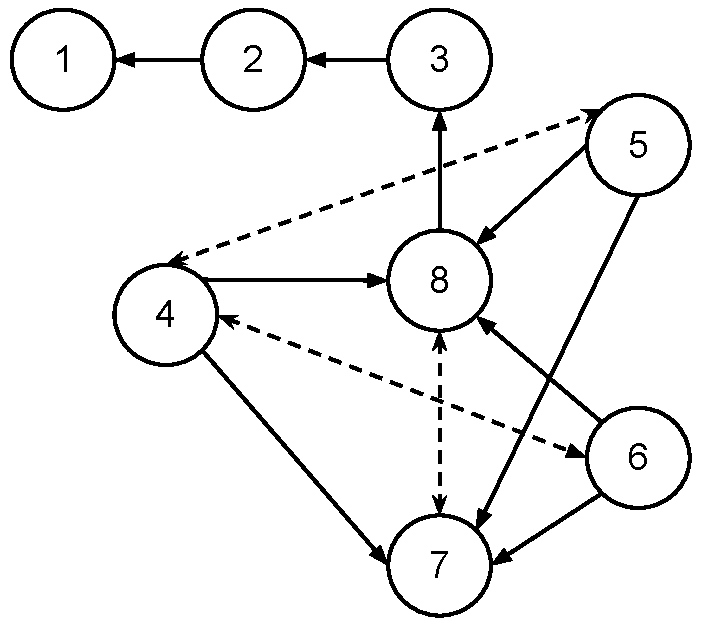
\includegraphics[width=\textwidth]{imgs/AbaloneNetwork}
\end{minipage}\hfill
\begin{minipage}[t]{0.45\linewidth}
 \vspace{0pt}
\centering
\begin{scriptsize}
\begin{tabular}{|l|}
\hline
The factor names\\
\hline
1. Length (longest shell) \\
2. Diameter\\
3. Height (with meat)\\
4. Whole weight  \\
5. Shucked weight (without shell)\\
6. Viscera weight (after bleeding) \\
7. Shell weight \\
8. Rings (indicating age)\\
\hline
\end{tabular}
\end{scriptsize}
\end{minipage}
\end{frame}

\section{Conclusion}
\begin{frame}{Wrap up}
\begin{itemize}
\item Causal Inference is a powerful tool for reasoning and predicting
\item Graphical model has a strong representation on causal conditions
\item Learning causation from data observation is totally feasible
\item Without additional information, only equivalence class can be achieved
\item Copula functions enable efficient parameter estimation
\item PICM based structure learning is also efficient
\item Promising experimental results show the interestingness of causal inference
\end{itemize}
\end{frame}

\section{References}
\begin{frame}{References}
\begin{thebibliography}{99}
\bibitem{Boas} J. Pearls,  Causality: Models, Reasoning, and Inference  \textit{Cambridge University Press}, \textbf{2000}.
\bibitem{Page} Joe Whittaker., Graphical Models in Applied Multivariate Statistics, \textit{John Wiley \& Sons}, Ltd, \textbf{2008}.
\bibitem{Page} Roger B. Nelsen, An Introduction to Copulas, \textit{Springer Science+Business Media}, Inc, \textbf{2006}.
\bibitem{Page} Jonas Peters, et al., Identifying Cause and Effect on Discrete Data using Additive Noise Models, \textit{JMLR}, Proceedings Track 9: 597-604, \textbf{2010}.
\end{thebibliography}
\end{frame}
\end{document}
